\documentclass[tikz,border=2pt]{standalone}
\usepackage{amsmath}
\usetikzlibrary{arrows.meta}
\begin{document}
% Open three-station network of the Example: external arrivals gamma=(3,1,0) per hour, routing
% P_12=1/3, P_13=2/3, P_23=1, P_31=0.2, exit P_30=0.8; traffic equations give lambda=(4,7/3,5).
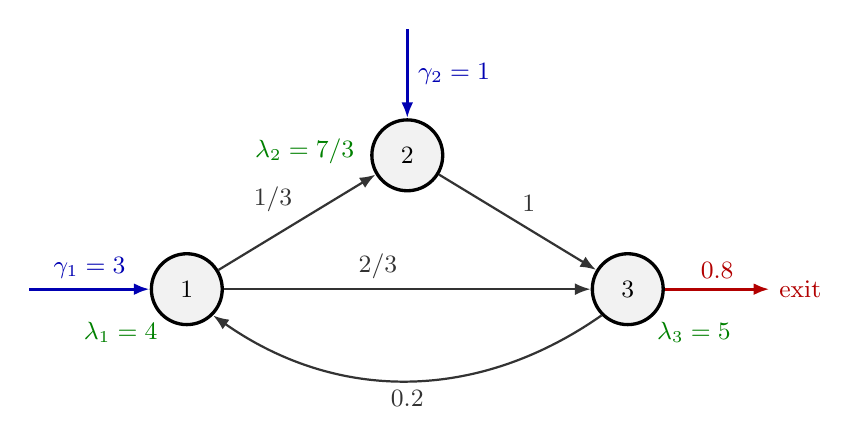
\begin{tikzpicture}[font=\small, >={Latex[length=2mm]},
  st/.style={circle, draw=black, very thick, fill=gray!10, minimum size=9mm}]
  \node[st] (s1) at (0,0) {$1$};
  \node[st] (s2) at (2.8,1.7) {$2$};
  \node[st] (s3) at (5.6,0) {$3$};
  % external arrivals
  \draw[->, very thick, blue!70!black] (-2.0,0) -- node[above] {$\gamma_1=3$} (s1.west);
  \draw[->, very thick, blue!70!black] (2.8,3.3) -- node[right] {$\gamma_2=1$} (s2.north);
  % routing
  \draw[->, thick, gray!40!black] (s1) -- node[above left, xshift=2pt] {$1/3$} (s2);
  \draw[->, thick, gray!40!black] (s1) -- node[above, pos=0.42] {$2/3$} (s3);
  \draw[->, thick, gray!40!black] (s2) -- node[above right, xshift=-2pt] {$1$} (s3);
  \draw[->, thick, gray!40!black] (s3.south west) to[bend left=35] node[below] {$0.2$} (s1.south east);
  % exit
  \draw[->, very thick, red!70!black] (s3.east) -- node[above] {$0.8$} (7.4,0);
  \node[red!70!black, anchor=west] at (7.4,0) {exit};
  % total arrival rates
  \node[green!50!black, anchor=north east] at (-0.25,-0.3) {$\lambda_1=4$};
  \node[green!50!black, anchor=east] at (2.25,1.75) {$\lambda_2=7/3$};
  \node[green!50!black, anchor=north west] at (5.85,-0.3) {$\lambda_3=5$};
\end{tikzpicture}
\end{document}
